\section{El modelo Transformer}

A finales del año 2017 se presentó un nuevo modelo que vino a revolucionar el área de Procesamiento
de Lenguaje Natural, El Transformer \cite{Vaswani}. Una de sus principales características es la
capacidad de procesar la información de alguna secuencia de forma paralela, caso contrario a las
Redes Neuronales Recurrentes, donde la información se procesa recurrentemente. Gracias a ello,
la capacidad de \textit{recuerdo} no se ve afectado por el problema de \textit{El desvanecimiento
del Gradiente} específicamente cuando el problema es trabajar con secuencias  bastante largas.

\textit{El Transformer} puede ser visto como otro modelo \textit{seq2seq} (Secuencia a Secuencia)
\ref{fig:trans_seq2sqe}, formado en por dos etapas, la primera encargada de codificar la información de entrada
y la segunda de decodificarla, pero la su principal característica es que aplica el mecanismos de
\textit{Self-Attention} para capturar las dependencias globales entre la entrada y la salida. Dada
una secuencia de entrada $X = (x_1, x_2, \dots, x_n )$ con $n$ como el tamaño de la secuencia,
el codificador produce una representación intermedia
$Z = (z_1, z_2, \dots, z_n)$ al igual que los modelos \textit{seq2seq}. El decodificador usa la
secuencia $Z$ para generar la secuencia de salida
$Y = (y_1, y_2, \dots, y_m)$ uno a la vez (en modo inferencia), con $m$ como el tamaño de la
secuencia de salida. Nótese, que el generar una salida a la vez el decodificador tiene que ser auto-regresivo.
Usa la salida anterior $y_{i-1}$ como entrada adicional para generar la siguiente salida $y_i$. Por
ello, durante entrenamiento el modelo es alimentado con entradas y salidas desfasadas en un tiempo.

\begin{figure}[ht!]
    \centering
    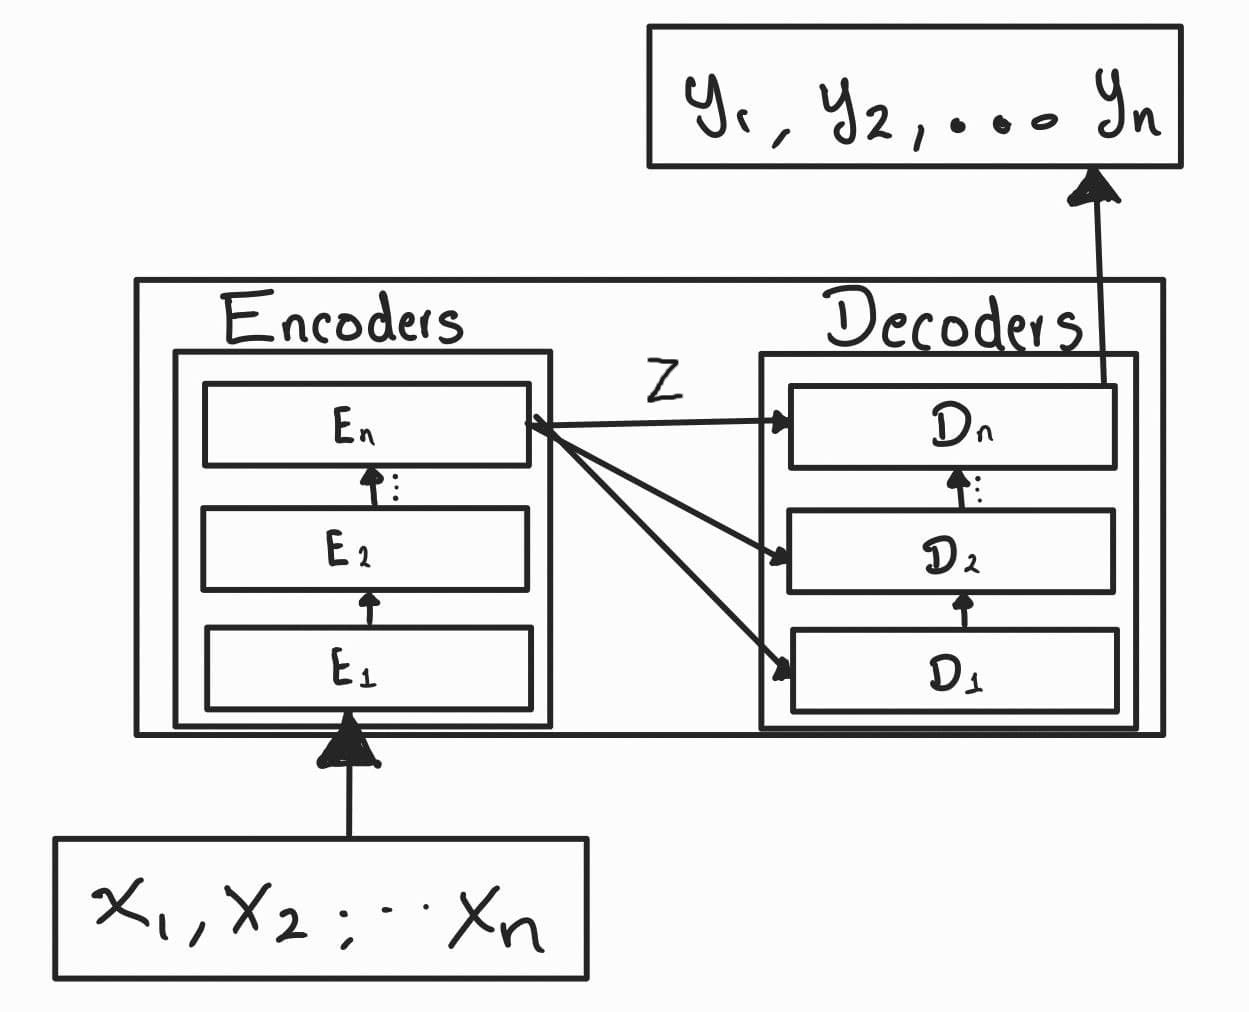
\includegraphics[width=0.4 \textwidth]{Chapters/1. Transformer/Figures/transformer/t_seq2seq.jpg}
    \caption{Modelo Transformer generalizado como modelo Secuencia a Secuencia}
    \label{fig:trans_seq2sqe}
\end{figure}

Poner ejemplo de Transformer en con la figura de arriba en tiempo de entrenamiento e inferencia aquí.

\subsection{El Codificador y Decodificador}

El \textit{Modelo Transformer} está formado por multiples codificadores  y decodificadores apilados e inter-conectados,
Como observamos en la figura \ref{fig:trans_seq2sqe}. El codificador consta de dos partes,
la primera de ellas aplica \textit{Self-Attention} múltiples veces sobre la misma entrada
(\textit{Multi-HeadSelf Attention}) y la segunda capa representada solo por una red
\textit{Feed-Forward} cuya entrada es la salida de la capa anterior.
Véase la figura \ref{fig:trans_encoder}.


\begin{figure}[ht!]
\centering
    \begin{minipage}{.4\textwidth}
        \centering
        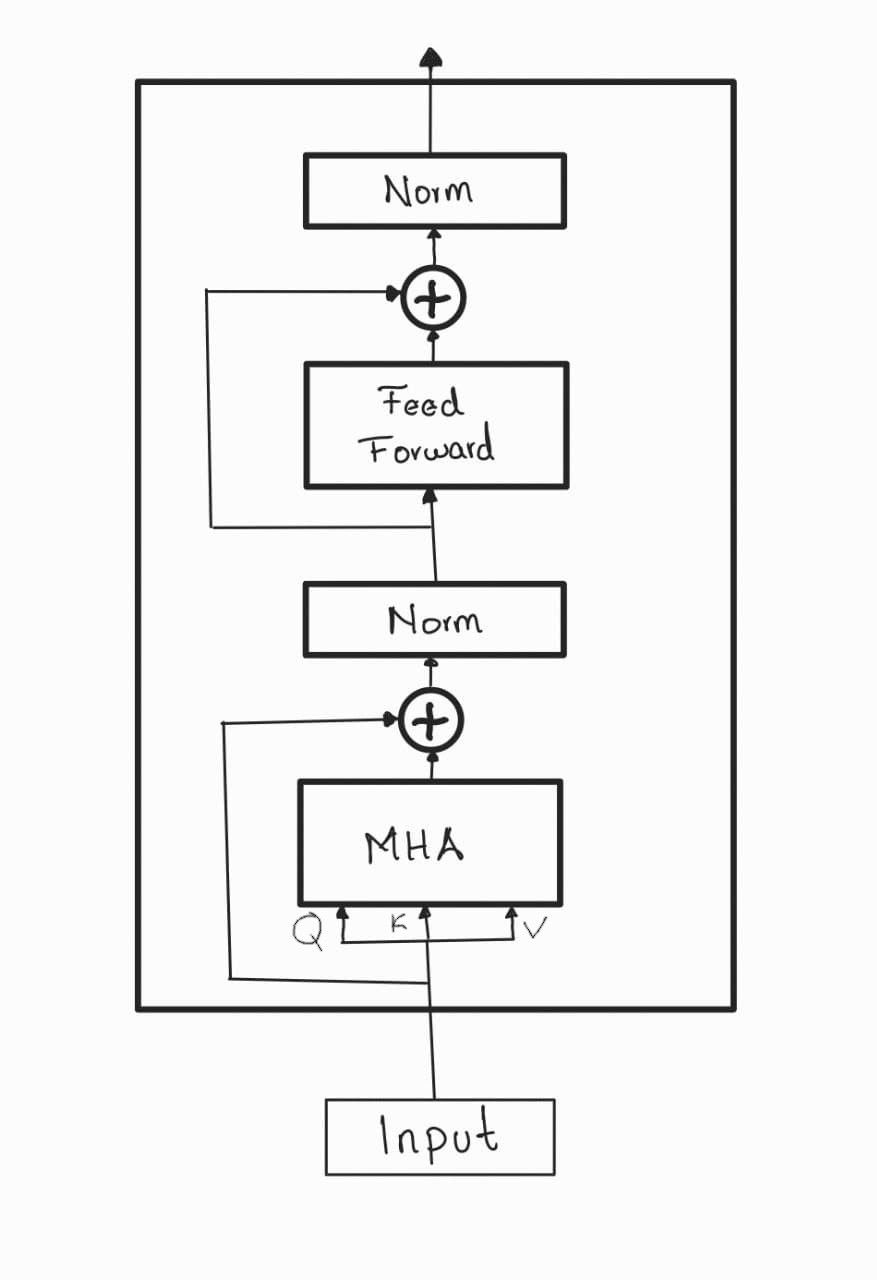
\includegraphics[width=0.7 \textwidth]{Chapters/1. Transformer/Figures/transformer/encoder.jpg}
    \end{minipage}
    \begin{minipage}{.5\textwidth}
        \begin{equation*}
            \begin{split}
                mha = MHA(X, X, X)\\
                norm = Norm( mha + X)\\
                f = FeedForward(norm)\\
                Encoder(X) = Norm(f + norm)
            \end{split}
            \label{eq:trans_enc}
        \end{equation*}
    \end{minipage}
    \caption{Etapa Codificadora del Modelo Transformer. Pseudocódigo}
    \label{fig:trans_encoder}
\end{figure}


El decodificador tiene una estructura similar al codificador con una etapa adicional intermedia
de \textit{Multi-Head Attention} aplicada sobre la salida de la pila de codificadores. También, la
primer capa de atención sufre un ligero cambio un su forma de operación, necesitando enmáscarar (al
momento en que se realiza el entrenamiento) la atención prestada del pasado al futuro. Esto es
debido a que el decodificador se encarga de generar una secuencia (en modo inferencia) uno a la vez
usando solamente la salida anterior y por tanto no tiene conocimiento de salidas futuras, observe
la figura \ref{fig:trans_te}.

\begin{figure}[ht!]
\centering
    \begin{minipage}{.4\textwidth}
        \centering
        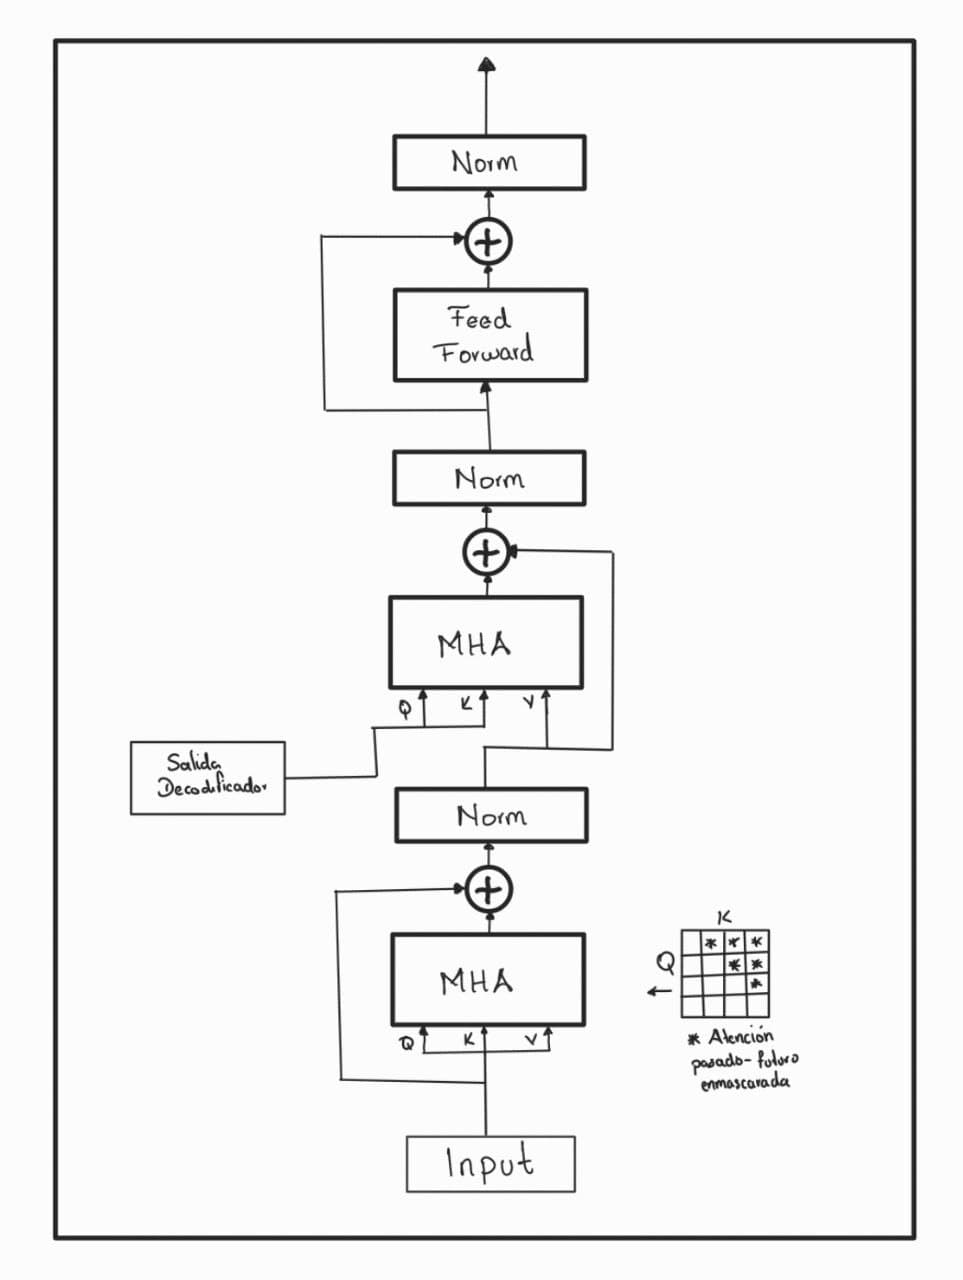
\includegraphics[width=1.0 \textwidth]{Chapters/1. Transformer/Figures/transformer/decoder.jpg}
    \end{minipage}
    \begin{minipage}{.5\textwidth}
        \begin{equation*}
            \begin{split}
                mha_1 = MHA(X, X, X)\\
                norm_1 = Norm( mha_1 + X)\\
                mha_2 = MHA(enc_{out}, enc_{out}, norm_1)\\
                norm_2 = Norm( mha_2 + X)\\
                f = FeedForward(norm_2)\\
                decoder(X) = Norm(f + norm_2)
            \end{split}
            \label{eq:trans_dec}
        \end{equation*}
    \end{minipage}
    \caption{Etapa Decodificadora del Modelo Transformer. Pseudocódigo}
    \label{fig:trans_decoder}
\end{figure}


\begin{figure}[ht!]
    \centering
    \begin{subfigure}[b]{0.49\textwidth}
        \centering
        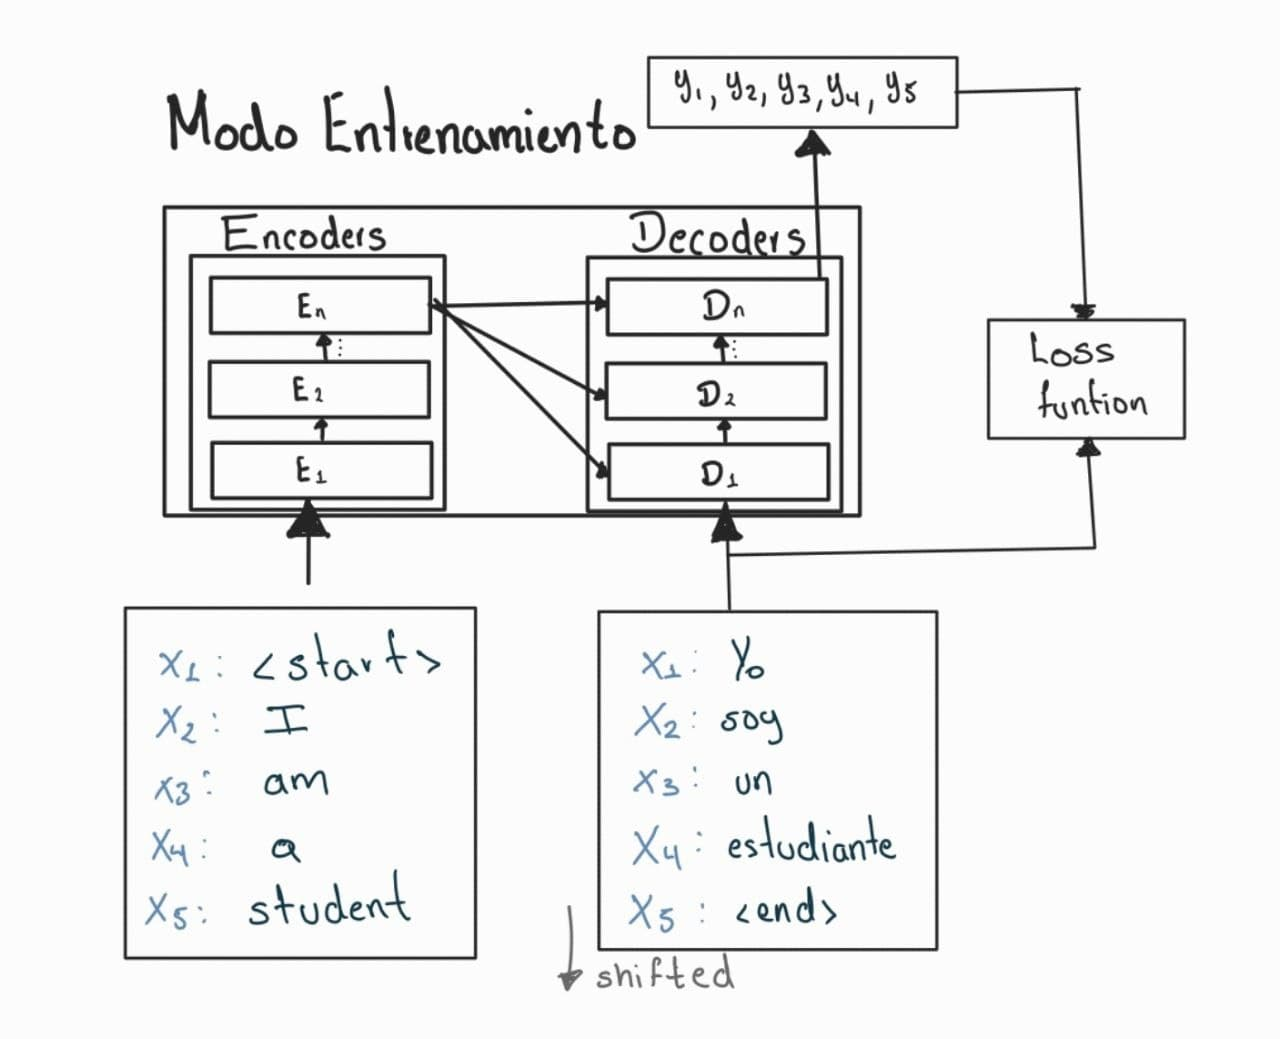
\includegraphics[width=1.0 \textwidth]{Chapters/1. Transformer/Figures/transformer/train.jpeg}
        \caption{Transformer modo entrenamiento. Las entradas en el decodificador son recorridas un
                 elemento en el futuro, con el fin de que aprende a predecir la siguiente palabra
                 dado un contexto previo y las salidas actuales en el momento de la evaluación.}
        \label{fig:trans_train}
    \end{subfigure}
    \begin{subfigure}[b]{0.49\textwidth}
        \centering
        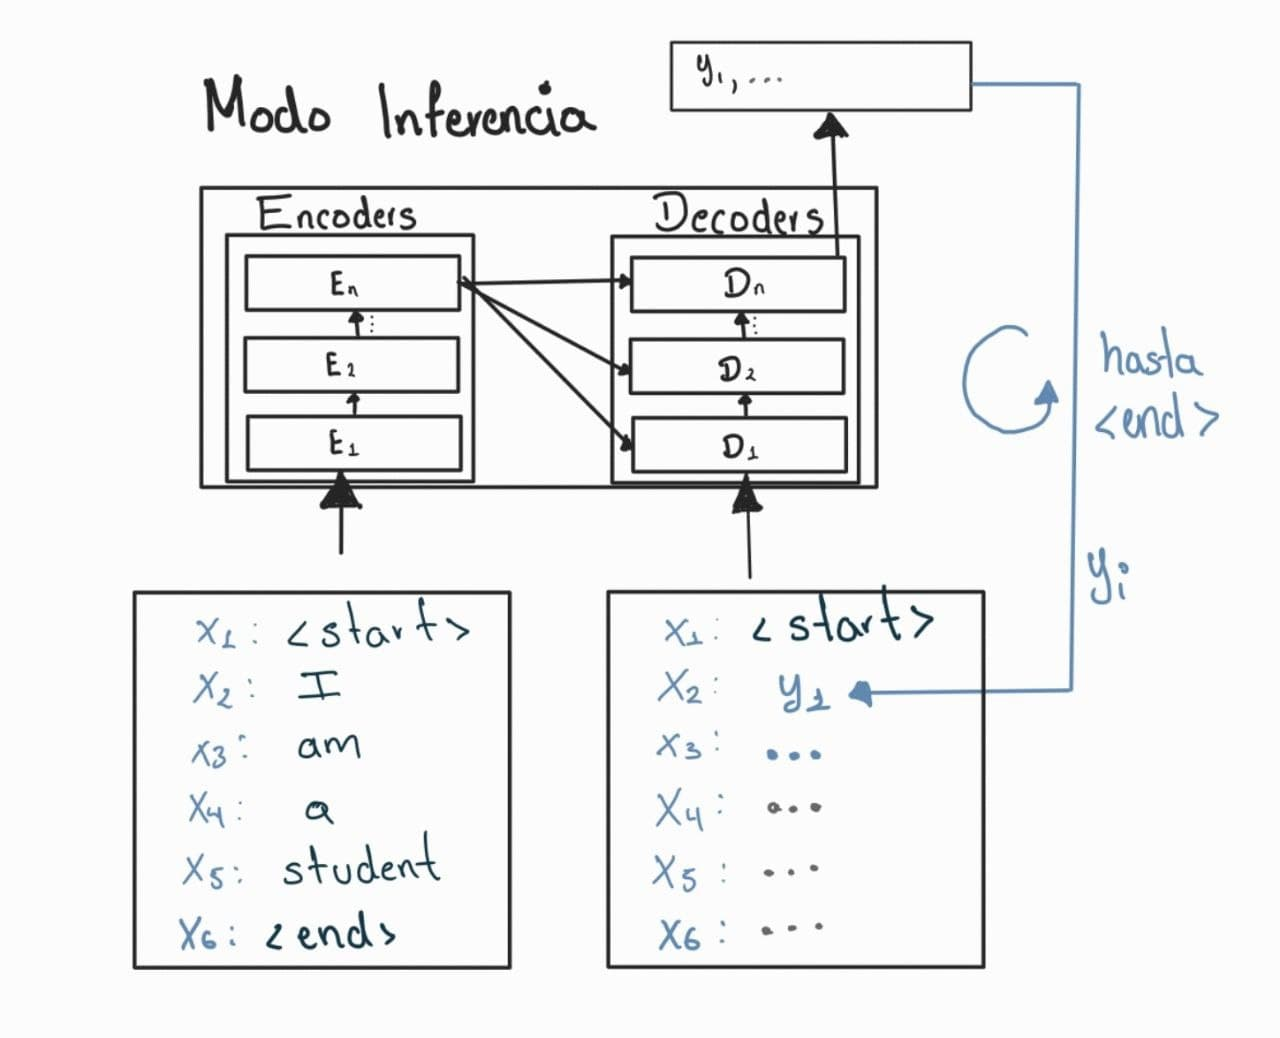
\includegraphics[width=1.0 \textwidth]{Chapters/1. Transformer/Figures/transformer/inference.jpg}
        \caption{Transformer modo inferencia. El decodificador funciona como un modelo auto-regresivo,
        usa sus predicciones hasta el tiempo $t$ para obtener el siguiente valor. En la primer iteración
        el decoder solo recibe el token de inicio de oración $<start>$ por lo que podrá predecir la primer
        palabra de la oración gracias a que fué entrenado con un desplazamiento hacia el futuro. En la siguiente
        iteración el nuevo token predicho es agregado como entrada al decodificador. El decodificador
        termina su predicción en el momento que el token $<end>$ es obtenido.}
        \label{fig:trans_eval}
    \end{subfigure}
    \caption{Esquema de entrenamiento e inferencia del modelo Transformer en un problema de
             Machine Translation.}
        \label{fig:trans_te}
\end{figure}


\subsection{Multi-Head Self-Attention}

En la sección \ref{section:att} se detalla una generalización de la atención y diversas variantes usadas
a lo largo de la literatura. El modelo original que introdujo a los Transformers usa en especial la variante
\textit{Scaled Dot-Product Attention}\cite{Vaswani}:

\begin{equation}
    Attention(q, k, v) = softmax(\frac{q k^\top}{\sqrt{d_k}}) v
    \label{eq:trans_att_gen}
\end{equation}

El Transformer está basado en la idea de de aplicar atención multiples veces, al usar varias cabezas
de atención, Multihead-Self-Attention (MHA), permite  al modelo conjuntamente atender a información
en distintas posiciones desde $h$ diferentes subespacios de representación. \ref{eq:mha}

\begin{equation}
    mha(Q, K, V) = Concat(head_1,head_2,head_3,..., head_h)W^O
    \label{eq:mha}
\end{equation}

Todas las cabezas de atención son concatenadas y resumidas para ser devueltas a las dimensiones del
espacio de entrada original, principalmente para mantener consistencia en las dimensiones de usadas
en cada etapa de codificación y decodificación del modelo a través de $W^O \in \mathbb{R}^{hd_v \times d_m}$.
$W^O$ es entrenado conjuntamente para aprender a resumir la información capturada por cada cabeza de
atención. $Q, K \in \mathbb{R}^{n \times d_{m}}$ y $V \in \mathbb{R}^{n \times d_{v}}$ es la representación
consulta, clave y valor de los embeddings de entrada de cada capa de atención del codificador y
decodificador como se observa en las figuras \ref{fig:trans_encoder} \ref{fig:trans_decoder}.
$n$ es el tamaño de la secuencia, $d_m$ y $d_v$ son los tamaño del embedding y $h$ el número de
cabezas de atención.

En el caso del modelo transformer tenemos un conjunto embeddings sobre las cuales se aplica atención,
si bien no representan necesariamente las consultas, llaves, y valores utilizados para la attention
generalizada,podemos obtener estas representaciones transportándo a sus espacios respectivos a través de alguna
transformación aprendida conjuntamente con el entrenamiento del modelo.

Por tanto, para el conjunto de Embeddings  $E_Q \in \mathbb{R}^{n \times d_m}$,
$E_K \in \mathbb{R}^{n \times d_m}$ y $E_V \in \mathbb{R}^{n \times d_v}$ donde $n$ es el número
embeddings, $d_m$ y $d_v$ son las dimensiones de cada uno, la atención en cada cabeza $i$ se calcula
como:

\begin{equation}
    \begin{split}
        Q_i = E_Q W_i^Q\\
        K_i = E_K W_i^K\\
        V_i = E_V W_i^K\\
    \end{split}
\end{equation}

\begin{equation}
\begin{split}
    head_i = Attention(Q_i, K_i, V_i) = softmax\Big(\frac{Q_i K_i^T}{\sqrt{d_k}}\Big) V_i
    \label{eq:trans_att}
\end{split}
\end{equation}

donde $W_i^Q$, $W_i^K$ $\in \mathbb{R}^{d_m \times d_k}$, $W_i^V$ $\in \mathbb{R}^{d_m \times d_v}$
y $d_k=d_v=d_m/h$.

el término de escalamiento $\sqrt{d_k}$ ayuda a evitar que la magnitud de los productos puntos calculados
entre cada consulta y llave crezcan demasiado, y que la función $softmax$ pueda ser más estable al evitar
regiones donde los gradientes son muy pequeños\cite{Vaswani}.


\subsection{Información Posicional}

En los modelos basados en \textit{Redes Recurrentes} la información se procesan uno a uno en cada paso de
tiempo. Los modelos basados en \textit{Transformers} procesan la información en conjunto, perdiendo
la noción de la temporalidad de los datos. Una solución es agregar dicha información perdida a través
de vectores que codifiquen el tiempo/posición de los datos sumándolos con los vectores de embeddings.
Estos vectores llamados \textit{Positional Encodings} \cite{DBLP:journals/corr/GehringAGYD17} siguen
un patrón en específico
que el modelo aprende a identificar y lo ayuda a determinar la posición de cada elemento de la secuencia
y por tanto calcular a qué distancia se encuentra cada uno de los demás.

Por lo regular se usa una onda senoidal y cosenoidal para lugares pares e impares, formando una progresión
geométrica desde $2\pi$ hasta $10000 \cdot 2\pi$ \ref{eq:trans_pos_enc}:

\begin{equation}
    \begin{split}
        PE(pos, 2i) = \sin(pos/10000^{2i/d_m})\\
        PE(pos, 2i+1) = \cos(pos/10000^{2i/d_m})
    \end{split}
    \label{eq:trans_pos_enc}
\end{equation}


\begin{figure}[ht!]
    \centering
    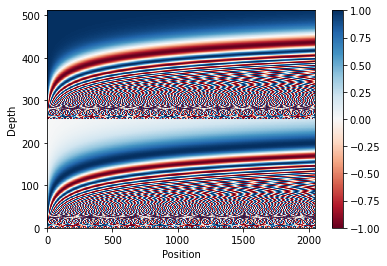
\includegraphics[width=0.5 \textwidth]{Chapters/1. Transformer/Figures/transformer/pos_enc.png}
    \caption{2000 Vectores de Positional Encoding con dimensiones de embedding=500.}
    \label{fig:trans_pos_enc}
\end{figure}

Poner una figura completa de todo el esquema del Transformer

\subsection{Problemas típicos en el entrenamiento de Transformers}
